\documentclass{article}
\usepackage{amsmath}
\usepackage{graphicx}
\usepackage{listings}
\usepackage{xcolor}

\title{Neural Genome Processing and Network Visualization}
\author{}
\date{}

\lstset{
    basicstyle=\ttfamily\small,
    backgroundcolor=\color{gray!10},
    breaklines=true,
    columns=fullflexible
}

\begin{document}

\maketitle

\section*{Overview}

This system models a simple feedforward neural structure with the following architecture:
\begin{itemize}
    \item $N_s = 8$ sensory (input) neurons
    \item $N_h = 4$ internal (hidden) neurons
    \item $N_a = 5$ action (output) neurons
    \item $N_c = 10$ connections encoded as 32-bit genes
\end{itemize}

\section*{Gene Structure}

Each gene is a 32-bit binary string (represented as 8 hex characters) encoding a single neural connection. The structure is:

\[
\underbrace{b_0}_{\text{source\_type}} \underbrace{b_{1-7}}_{\text{source\_id}} \underbrace{b_8}_{\text{sink\_type}} \underbrace{b_{9-15}}_{\text{sink\_id}} \underbrace{b_{16-31}}_{\text{weight}}
\]

\begin{itemize}
    \item \textbf{source\_type}: $0$ for sensory neuron, $1$ for internal neuron
    \item \textbf{sink\_type}: $0$ for internal neuron, $1$ for action neuron
    \item \textbf{weight}: 16-bit signed integer mapped to real value in $[-4.0, 4.0]$
\end{itemize}

\section*{Activation Propagation}

The network computes values as follows:

\begin{enumerate}
    \item Propagate values from sensory neurons to internal or action neurons.
    \item Store connections from internal $\to$ internal and internal $\to$ action for delayed execution.
    \item Evaluate internal $\to$ internal, then apply $\tanh$ activation to internal layer.
    \item Evaluate internal $\to$ action, then apply $\tanh$ to action layer.
\end{enumerate}

Finally, the softmax of the action layer is used to probabilistically select an action.

\[
\text{softmax}(x_i) = \frac{e^{x_i}}{\sum_j e^{x_j}}
\]

\section*{Example Brain Structure}

An example graph of the neural architecture from a randomly generated genome is shown below. Connections are color-coded:

\begin{itemize}
    \item \textcolor{blue}{Blue}: excitatory ($w > 0$)
    \item \textcolor{red}{Red}: inhibitory ($w < 0$)
\end{itemize}

\begin{figure}[h!]
    \centering
    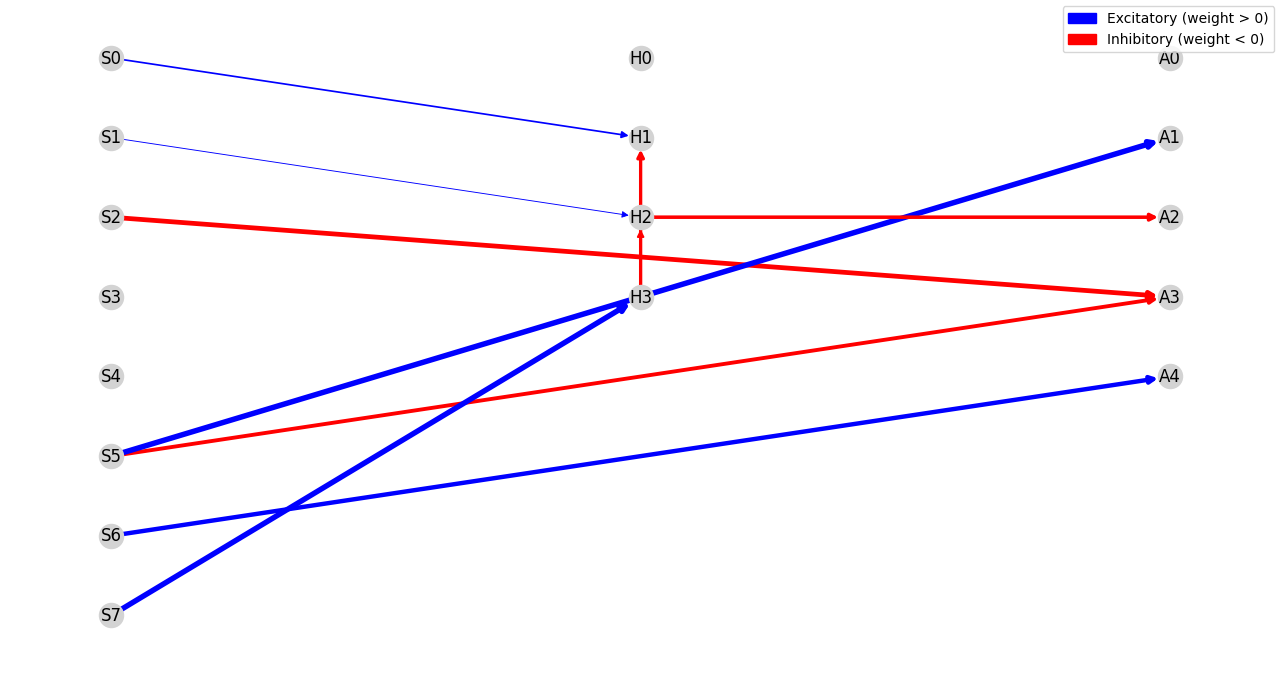
\includegraphics[width=0.9\textwidth]{brain_structure.png}
    \caption{Graphical representation of the neural genome structure}
\end{figure}

\end{document}
